%%%% fatec-article.tex, 2024/03/10

%% Classe de documento
\documentclass[
  a4paper,%% Tamanho de papel: a4paper, letterpaper (^), etc.
  12pt,%% Tamanho de fonte: 10pt (^), 11pt, 12pt, etc.
  english,%% Idioma secundário (penúltimo) (>)
  brazilian,%% Idioma primário (último) (>)
]{article}

%% Pacotes utilizados
\usepackage[]{fatec-article}
\usepackage{setspace}
\usepackage{float}

\Author{1}{Name={Vinicius Souza Ramos\\ Paulo Cesar Pedro Candiani \\ João Pedro Kuzinor de Lima \\ Gabriel Guimarães Carneiro \\ João Pedro Dias Barreto}}

\Author{2}{Name={\{ vinicius.ramos31@fatec.sp.gov.br \}\\ \{ paulo.candiani@fatec.sp.gov.br \} \\ \{ joao.lima135@fatec.sp.gov.br \} \\ \{ gabriel.carneiro3@fatec.sp.gov.br \} \\ \{ joao.barreto4@fatec.sp.gov.br \}}}

%% Definição das palavras-chaves/keywords
\Keyword{1}{Pecuária leiteira}{Dairy farming}
\Keyword{2}{Bubalinos}{Buffaloes}
\Keyword{3}{Manejo de rebanho}{Herd management}
\Keyword{4}{Produção de leite}{Milk production}

%%%% Resumo no idioma primário (brazilian)
\begin{Abstract}[brazilian]%% Idioma (brazilian ou english)
  O manejo eficiente de bubalinos é essencial para o desenvolvimento da pecuária leiteira, especialmente em regiões que dependem economicamente da produção de leite. No entanto, o controle e a análise de dados de rebanhos ainda são realizados de forma manual em muitas propriedades, o que compromete a produtividade e a tomada de decisões estratégicas. Este estudo propõe o desenvolvimento de uma plataforma digital para auxiliar na gestão do rebanho bubalino, com foco na produção de leite, utilizando tecnologias web e dispositivos móveis. A solução integra uma aplicação web e uma aplicação móvel conectadas a uma API desenvolvida em Node.js, responsável pela comunicação com a base de dados. A plataforma permite o registro e a visualização de informações detalhadas sobre os animais, como estágio de maturidade, raça, sexo e desempenho na lactação, além de oferecer recursos gráficos para facilitar a análise de produtividade. A proposta visa modernizar o processo de manejo, apoiar a tomada de decisões no campo e promover um controle mais inteligente da produção leiteira.
\end{Abstract}

%%%% Resumo no idioma secundário (english)
\begin{Abstract}[english]%% Idioma (brazilian ou english)
  Efficient buffalo management is essential for the development of dairy farming, especially in regions that are economically dependent on milk production. However, herd data control and analysis are still carried out manually on many farms, which compromises productivity and strategic decision-making. This study proposes the development of a digital platform to assist in the management of buffalo herds, focusing on milk production, using web and mobile technologies. The solution integrates a web application and a mobile application connected to an API developed in Node.js, which is responsible for communication with the database. The platform allows the registration and visualization of detailed information about the animals, such as maturity stage, breed, sex, and lactation performance, in addition to offering graphical resources to facilitate productivity analysis. The proposal aims to modernize the management process, support decision-making in the field, and promote smarter control of milk production.
\end{Abstract}

%% Processamento de entradas (itens) do índice remissivo (makeindex)
\makeindex%

%% Arquivo(s) de referências
\addbibresource{fatec-article.bib}

%% Início do documento
\begin{document}

% Seções e subseções
%\section{Título de Seção Primária}%

%\subsection{Título de Seção Secundária}%

%\subsubsection{Título de Seção Terciária}%

%\paragraph{Título de seção quaternária}%

%\subparagraph{Título de seção quinária}%

\section*{Introdução}%
\label{sect:intro}
A primeira introdução de búfalos no Brasil teria ocorrido por volta de 1895, trazidos por condenados foragidos da Guiana Francesa em um barco que aportou na costa norte da Ilha do Marajó. A introdução mais documentada, no entanto, ocorreu por volta de 1902, com uma importação feita por Bertino Lobato de Miranda para sua Fazenda São Joaquim, localizada às margens do rio Ararí, também na Ilha do Marajó. Esses búfalos eram pretos, de procedência italiana \cite{ABCB2016}. Com o passar dos anos, diversas outras importações foram realizadas por criadores do Marajó, do Baixo Amazonas, do Nordeste, do Sul e de Minas Gerais. Atualmente, o rebanho bubalino no Brasil é de aproximadamente 1.672.956 cabeças \cite{IBGE2023}, distribuídas entre diversos estados.

A criação de búfalos é de grande importância para o atendimento da demanda alimentar (leite e carne) e também para a economia, tanto no Brasil quanto no mundo. Esses animais apresentam vantagens em relação a outros ruminantes domésticos, principalmente no que diz respeito à rusticidade, à capacidade de aproveitamento de alimentos de baixa qualidade, à adaptação a terrenos alagadiços e às variadas condições climáticas e de manejo \cite{EMBRAPA2019}.

O leite de búfala possui características únicas que o diferenciam do leite de vaca. Segundo Marques, em seu livro Criação de Búfalos, na elaboração de laticínios, o leite bubalino apresenta um rendimento industrial cerca de 40\% superior ao leite bovino. Além disso, possui 33\% menos colesterol, 48\% mais proteína, 59\% mais cálcio e 47\% mais fósforo. Por conter maior teor de gordura, é necessária uma menor quantidade de leite para a produção de produtos como manteiga e queijos, quando comparado ao leite de vaca \cite{Embrapa1998}. Com base nessas informações, as búfalas são consideradas excelentes produtoras de leite. Elas podem atingir médias superiores a 7 litros de leite por fêmea/dia, durante lactações de aproximadamente 270 dias. No entanto, a média nacional não ultrapassa 5 litros por fêmea/dia, em lactações de cerca de 250 dias \cite{Embrapa1998}. Para aumentar essa produtividade, práticas como a seleção de matrizes (definindo um mínimo produtivo para permanência no rebanho), a seleção de reprodutores (com foco em valor genético para produção leiteira), o manejo adequado e os cuidados sanitários são essenciais.

Para embasar este projeto, realizaram-se pesquisas de campo em propriedades voltadas à produção de leite de búfala, localizadas na região do Vale do Ribeira. Optou-se pela metodologia de pesquisa qualitativa, com o objetivo de compreender as particularidades de diferentes realidades produtivas. Foram entrevistados dois produtores com perfis distintos, um com um rebanho de 12 cabeças e outro com mais de 400, além de um médico-veterinário especializado, atuante em uma indústria de laticínios da região. Este profissional presta atendimento a diversos fornecedores da empresa, oferecendo uma visão ampla sobre os padrões e cuidados adotados na criação de bubalinos.

A pesquisa com os produtores revelou que ambos não utilizam softwares específicos para o manejo de bubalinos. Ao ser feita a pergunta: “Existe algum software específico utilizado para o gerenciamento do manejo de fazenda com foco na lactação de búfalos? Se sim, qual?”, ambos responderam que desconhecem a existência de um sistema específico para o manejo de bubalinos. Eles mencionaram conhecer plataformas desenvolvidas para o manejo de bovinos, o que não se mostra totalmente efetivo, pois, quando se trata de informações reprodutivas, o tempo de gestação do bovino é de cerca de 9 meses (SILVA, 2020), enquanto o dos bubalinos é de aproximadamente 10 meses (EMBRAPA, 2007). Dessa forma, há uma diferença média de cerca de 30 dias, o que faz com que softwares com valores pré-definidos acusassem que as búfalas estão com a reprodução atrasada.

Seguindo a mesma linha de investigação, foi questionado o interesse em utilizar um sistema específico para auxiliar o manejo: “Se existisse um software específico para o gerenciamento do manejo de fazendas com foco na lactação de búfalos, que possuísse funcionalidades para identificar os búfalos com desempenho abaixo da média e para acompanhar as informações sanitárias, zootécnicas e de lactação, como ele poderia impactar a gestão e melhorar os resultados da propriedade?”. Ambos demonstraram interesse em uma solução voltada ao setor, reconhecendo que a adoção de um sistema digital poderia tornar a avaliação do desempenho da propriedade mais precisa e reduzir perdas de informações importantes.

Durante as entrevistas, também foi feita a pergunta: “Na sua opinião, quais funcionalidades seriam necessárias para que um sistema atendesse à sua forma de trabalho?”. O objetivo foi identificar possíveis lacunas na proposta atual do sistema, permitindo o planejamento de futuras atualizações. As respostas indicaram duas sugestões relevantes: (1) a implementação de uma visualização da árvore genealógica dos animais, considerada essencial para o controle das matrizes presentes na propriedade, visando sempre as que mais produzem leite; (2) uma funcionalidade que possibilite identificar rapidamente o animal por meio do celular, exibindo seu prontuário com todas as informações disponíveis, sendo que esta última já estava prevista na proposta do sistema em desenvolvimento.

Além das propriedades voltadas à produção de leite, também foi realizada uma entrevista com representantes de um Instituto de Zootecnia localizado na mesma região. Durante a entrevista, foi possível observar que o controle do rebanho, no instituto, é realizado por meio de planilhas eletrônicas separadas por áreas temáticas, como pesagem dos animais, produção de leite, registros de cruzamentos, tratamentos e separação de grupos. Cada planilha contém múltiplas abas correspondentes aos anos de registro, exigindo a repetição manual de informações entre diferentes arquivos e períodos. Essa estrutura fragmentada torna o processo massivo e suscetível a erros, além de dificultar a manutenção de um histórico consolidado dos dados do rebanho.

Este projeto está alinhado às áreas temáticas definidas pelo Fórum de Pró-Reitores de Extensão das Universidades Públicas Brasileiras (FORPROEX), atendendo aos eixos de Meio Ambiente (5) e Tecnologia (7). Também contempla as linhas de extensão voltadas ao Desenvolvimento de Produtos (7), Desenvolvimento Tecnológico (10), Gestão do Trabalho (22) e Saúde Animal (43). Tal enquadramento reforça o compromisso da proposta com os princípios da extensão universitária, contribuindo para a integração entre conhecimento científico, demandas sociais e inovação prática no setor agropecuário \cite{FORPROEX}.

\section*{OBJETIVO} \label{sect:obj}

Desenvolver uma aplicação multiplataforma voltada à otimização e ao apoio da gestão de bubalinos em propriedades produtoras de leite, centralizando informações zootécnicas, sanitárias, reprodutivas e produtivas, e incorporando técnicas de Inteligência Artificial para previsão da produção de leite e geração de alertas automatizados. A plataforma fornecerá ao produtor uma visão integrada do desempenho e saúde do rebanho, contribuindo para a eficiência produtiva, redução de perdas de informação e aprimoramento das estratégias de seleção, reprodução e comercialização do leite bubalino.

Para atender às necessidades dos produtores, o sistema implementará funcionalidades que permitam o acompanhamento individualizado de cada animal e o gerenciamento de indicadores-chave de desempenho da fazenda. Entre as principais funções previstas, destacam-se:

\begin{enumerate}
    \item Registrar dados zootécnicos, métricas corporais dos animais, permitindo acompanhamento individual e monitoramento do desenvolvimento do rebanho.
    \item Controlar informações sanitárias, incluindo vacinas, medicamentos e tratamentos, garantindo rastreabilidade e saúde do rebanho.
    \item Gerir o ciclo reprodutivo, acompanhando cruzamentos, gestações e partos.
    \item Monitorar a produção de leite, registrando volumes por animal durante o ciclo produtivo, para análise de desempenho.
    \item Implementar recursos de Inteligência Artificial para prever a produção individual de leite das fêmeas, classificando o potencial produtivo e gerando alertas inteligentes para suporte à tomada de decisão.
    \item Gerir a produção e comercialização do leite, controlando volumes vendidos, quantidades aprovadas e reprovadas, além de informações sobre manejo, como distribuição de piquetes e confinamentos.
\end{enumerate}


Essas funcionalidades, integradas em uma única plataforma digital, visam fornecer ao produtor informações precisas e acessíveis, facilitando a tomada de decisões estratégicas e promovendo a modernização da gestão das propriedades que visão a bubalinocultura.

\section*{ESTADO DA ARTE} \label{sect:estadoarte}

Com o intuito de apoiar o desenvolvimento deste projeto, foi realizada uma pesquisa sobre trabalhos e projetos correlatos. Observou-se que muitos estudos focam na fase de lactação dos bovinos, tema que, embora semelhante ao abordado neste trabalho, apresenta algumas diferenças em sua abordagem e implementação. Ainda assim, esses projetos fornecem uma base valiosa, uma vez que reforçam a necessidade da aplicação de sistemas informatizados no setor pecuário. A adoção da tecnologia se mostra uma excelente alternativa às práticas ainda comuns em muitas propriedades, como o uso de anotações físicas e planilhas em softwares genéricos. Dessa forma, a literatura existente valida a proposta deste sistema, ao destacar os benefícios da informatização no manejo leiteiro.

O primeiro estudo analisado foi apresentado por \cite{SCHAFFER2021}, que desenvolveu uma plataforma web para o gerenciamento de bovinos, com o intuito de substituir métodos tradicionais utilizados pelos produtores rurais, como planilhas e registros em papel. O sistema foi implementado utilizando HTML, CSS, JavaScript, PHP e a biblioteca Bootstrap, além de empregar o banco de dados MySQL por meio do pacote XAMPP, disponibilizando uma interface responsiva que pode ser acessada também por dispositivos móveis. Entre suas principais funcionalidades, destacam-se o controle detalhado das informações zootécnicas dos animais, incluindo histórico de saúde, dados reprodutivos para fêmeas, e atributos cadastrais como sexo, raça e data de nascimento. O sistema permite ainda a atualização e remoção de registros individualmente, bem como a visualização do histórico sanitário de cada bovino, promovendo maior organização e segurança no gerenciamento do rebanho. Apesar disso, o projeto apresenta limitações, principalmente no que diz respeito à indisponibilidade de funcionamento em modo offline, impossibilitando seu uso em ambientes rurais sem conectividade a uma rede de internet. Além disso, o artigo destaca que melhorias futuras poderiam incluir a adoção de um servidor de banco de dados mais robusto, visando ampliar a escalabilidade, segurança e estabilidade da solução em cenários reais de produção.

O segundo projeto analisado foi o Trabalho de Conclusão de Curso desenvolvido por \cite{Pamella2017}, que consistiu na criação de um sistema voltado ao controle de rebanho bovino leiteiro. O objetivo principal foi oferecer uma solução tecnológica alinhada às reais necessidades do campo, prezando por praticidade, agilidade e eficiência no manejo dos animais. O sistema foi implementado utilizando a linguagem de programação Java, com desenvolvimento realizado na IDE NetBeans e com armazenamento de dados em um banco relacional SQL Server. Entre suas funcionalidades, destacam-se o controle reprodutivo, a pesagem de leite, a visualização dinâmica de dados e a geração de relatórios. A aplicação foi testada na fazenda Dois Irmãos, onde foram observados resultados significativos. O controle reprodutivo dos bovinos tornou-se mais organizado e eficiente, o processo de pesagem de leite foi automatizado, reduzindo erros comuns no método manual, e as necessidades específicas do proprietário, sobretudo no que se refere à geração de relatórios, foram plenamente atendidas. Além disso, a acessibilidade e a variedade de formas de visualização dos dados facilitaram a administração da propriedade e contribuíram para a tomada de decisões estratégicas. Os resultados obtidos evidenciam o potencial da tecnologia como ferramenta essencial para o avanço da pecuária leiteira.

O terceiro estudo relevante é apresentado por \cite{LIMA2023}, que propôs o desenvolvimento de um web aplicativo denominado \textit{Leite Cowtrol}, voltado ao controle da produção leiteira e gestão reprodutiva de gado leiteiro. O trabalho surgiu a partir da identificação de limitações presentes em soluções já existentes no mercado, como interfaces pouco intuitivas, inconsistências em registros de inseminação e a ausência de ferramentas que auxiliem diretamente na tomada de decisão do produtor. Para sua implementação, foram utilizadas tecnologias como HTML5, CSS3, JavaScript e o framework React.js, escolhidos por sua compatibilidade com dispositivos móveis, responsividade e ecossistema consolidado. O armazenamento de dados foi realizado em MySQL, complementado pelo uso de \textit{LocalStorage} para manter persistência local e personalização na experiência do usuário. Entre as funcionalidades propostas, destacam-se o gerenciamento do ciclo de vida dos animais e o monitoramento da produção de leite, recursos fundamentais para melhorar a organização do rebanho e otimizar a produtividade. Embora o protótipo tenha demonstrado potencial para atender aos requisitos definidos e contribuir para o aprimoramento dos envolvidos no projeto, o estudo apresenta limitações importantes, como a ausência de testes práticos em propriedades rurais, impossibilitando a validação de sua eficácia em cenários reais e restringindo a análise de desempenho em condições operacionais.

Observa-se que ambos os trabalhos analisados possuem como foco exclusivo a gestão de rebanhos bovinos leiteiros, não contemplando particularidades de outras espécies, como bubalinos, que apresentam características produtivas, sanitárias e reprodutivas distintas. Além disso, as soluções propostas ainda demonstram limitações consideráveis no uso prático, como a dependência de conectividade constante, o predomínio de aplicações web ou desktop que restringem a mobilidade e dificultam o registro de informações em campo, bem como a ausência de validação em propriedades rurais reais, o que compromete a análise de desempenho sob condições operacionais. Outro aspecto observado é a falta de discussão sobre hospedagem e infraestrutura de implantação, não abordando custos operacionais, escalabilidade dos sistemas ou requisitos de disponibilidade.  Também se destaca a inexistência de mecanismos baseados em inteligência artificial capazes de apoiar a tomada de decisões estratégicas, detecção precoce de problemas sanitários ou geração de previsões produtivas. Nesse contexto, o presente projeto busca suprir essas lacunas ao propor uma solução híbrida composta por plataforma web e aplicativo mobile, priorizando mobilidade, acessibilidade e autonomia do usuário. Aliada a isso, a integração de modelos de aprendizado de máquina constitui um diferencial técnico relevante, permitindo a emissão de alertas sanitários e predições de produção leiteira, ampliando o suporte ao manejo e favorecendo decisões fundamentadas em evidências.

\section*{METODOLOGIA} \label{sect:metodologia}

A plataforma proposto, denominado Buffs, consiste no desenvolvimento de uma aplicação multiplataforma composta por versões web e mobile, atuando como o principal meio de interação entre o usuário e os dados da propriedade. A aplicação disponibiliza uma interface gráfica intuitiva, permitindo o registro, consulta e análise das informações cadastradas, assegurando controle preciso e acompanhamento em tempo real do rebanho, desde que alimentada continuamente pelo usuário. Cada versão desempenha um papel complementar: a aplicação mobile \Cref{fig:mobile}, direcionada a funcionários e veterinários, adota princípios de interface enxuta, priorizando agilidade no lançamento de informações e feedback visual imediato durante o trabalho em campo. Por sua vez, a plataforma web \Cref{fig:web}, voltada a gestores e proprietários, oferece visão abrangente e detalhada dos dados, permitindo análises estratégicas em ambiente de escritório. Ambas as versões atuam de forma integrada, promovendo sincronização automática e garantindo consistência das informações em tempo real, independentemente do dispositivo utilizado.

\newpage

\begin{figure}[!h]
\centering
\caption{Telas Aplicativo Mobile}%
\label{fig:mobile}
\begin{subfigure}[b]{0.25\textwidth}
    \centering
    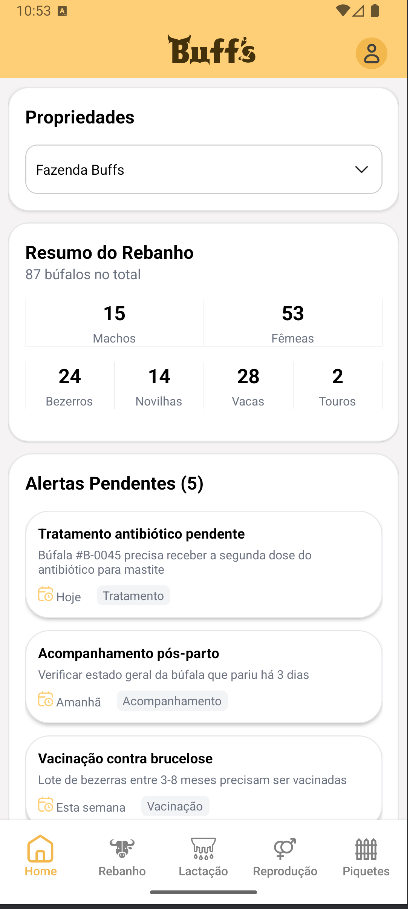
\includegraphics[width=\textwidth]{mobile/home}
    \caption{Tela inícial}
    \label{fig:web_coleta}
\end{subfigure}
\hspace{2cm}
\begin{subfigure}[b]{0.25\textwidth}
    \centering
    \includegraphics[width=\textwidth]{mobile/rebanho}
    \caption{Visualização do rebanho}
    \label{fig:web_piquete}
\end{subfigure}
\SourceOrNote{Autoria Própria (2025)}
\end{figure}


\begin{figure}[!h]
\caption{Exemplos de telas da plataforma web, mostrando indicadores, piquetes e inventário do rebanho}
\centering
\label{fig:web}
\begin{subfigure}[b]{0.424\textwidth}
    \centering
    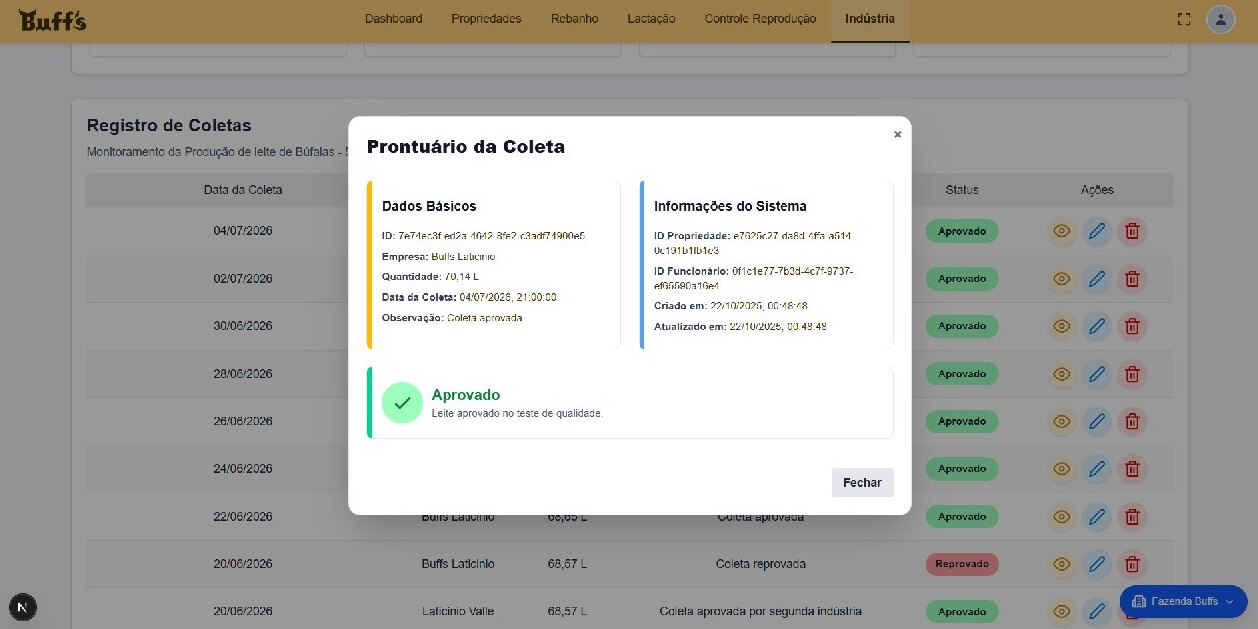
\includegraphics[width=\textwidth]{web/coleta}
    \caption{Feedback de uma coleta}
    \label{fig:web_coleta}
\end{subfigure}
\hfill
\begin{subfigure}[b]{0.424\textwidth}
    \centering
    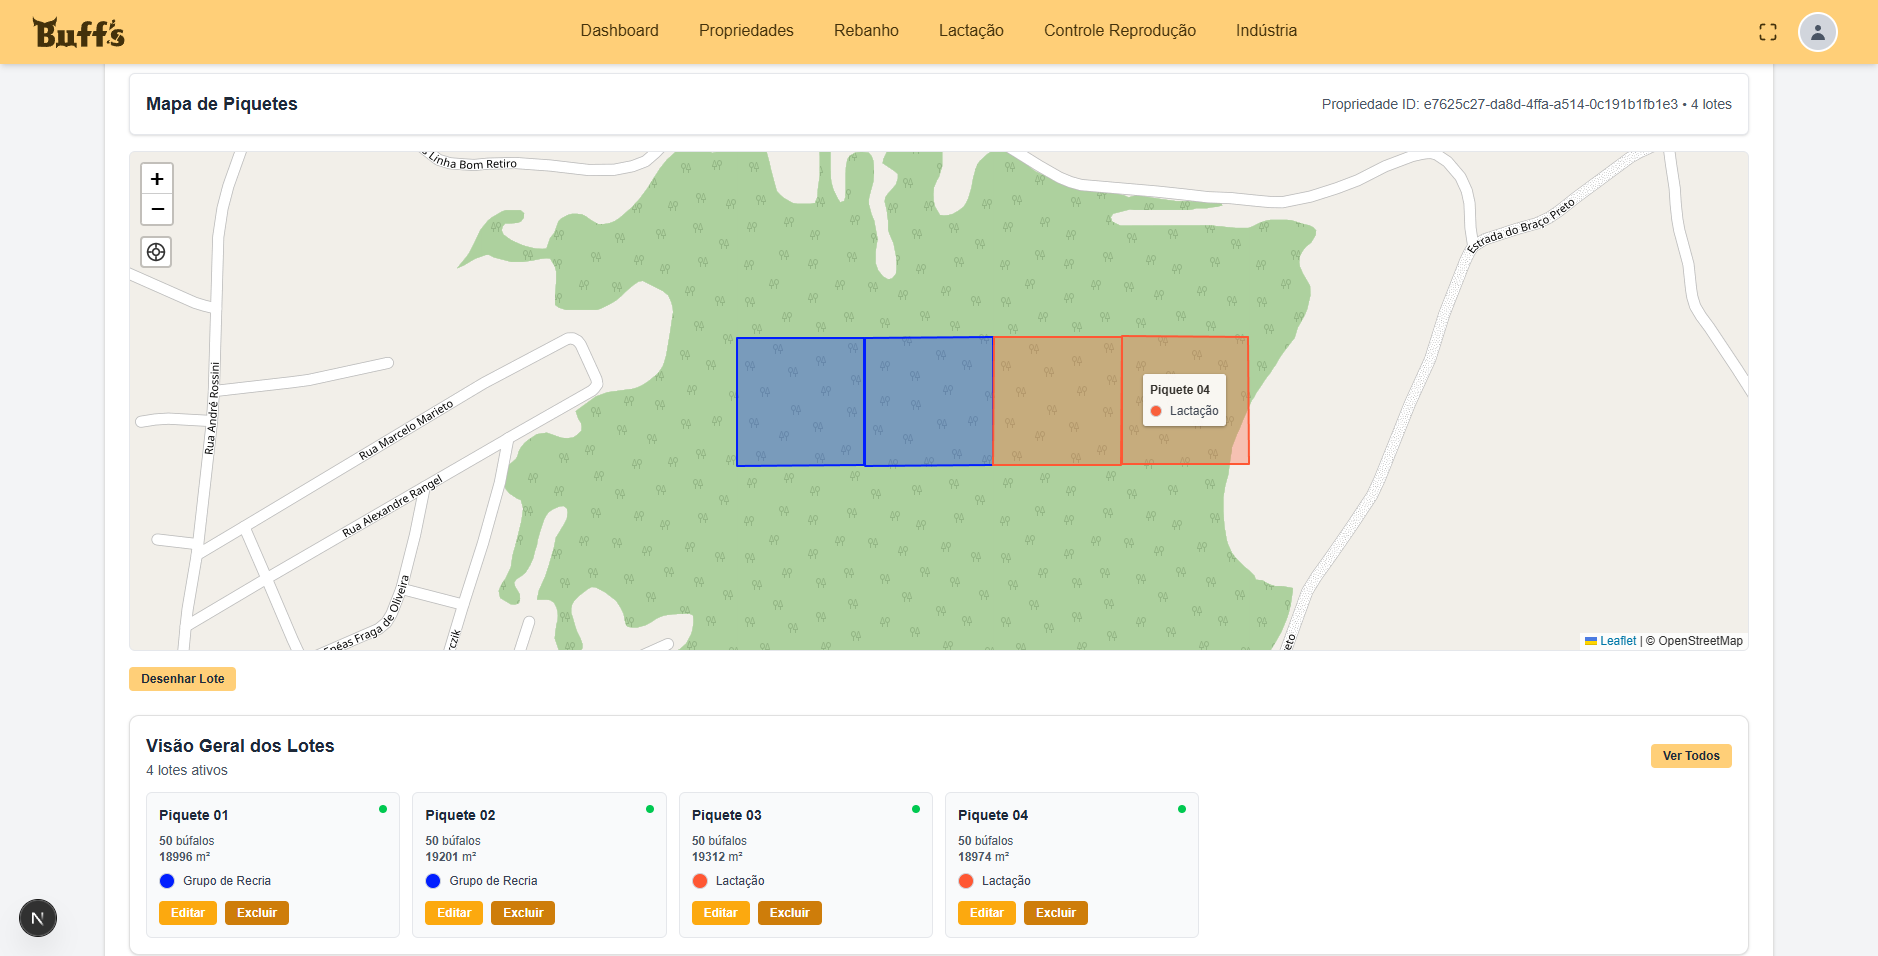
\includegraphics[width=\textwidth]{web/piquete}
    \caption{Visualização de piquetes}
    \label{fig:web_piquete}
\end{subfigure}

\vspace{0.5cm} % Espaço entre linhas

\begin{subfigure}[b]{0.45\textwidth}
    \centering
    \includegraphics[width=\textwidth]{web/rebanho}
    \caption{Visualização do rebanho}
    \label{fig:web_rebanho}
\end{subfigure}

\label{fig:web_exemplos}
\SourceOrNote{Autoria Própria (2025)}
\end{figure}

\newpage

No \Cref{fcht:fluxograma1} é possivel verificar o fluxo que o Funcionário/Veterinário vão seguir, ao acessa o sistema por meio do aplicativo móvel, por onde realiza a inserção e consulta de informações zootécnicas, sanitárias, reprodutivas e produtivas. Durante o registro de uma nova ordenha, o sistema ativa automaticamente a inteligência artificial(IA) generativa Gemini, que analisa os dados inseridos e identifica descrições compatíveis com mastite. Quando uma ocorrência é constatada, a IA classifica seu nível de gravidade, emitindo alertas que orientam o usuário quanto à urgência de intervenção. Essa abordagem automatizada reduz o risco de omissões, padroniza decisões e agiliza o tratamento clínico, garantindo maior confiabilidade ao processo. As inserções de dados realizadas pelo aplicativo são enviadas à Interface de Programação de Aplicações, do inglês \textit{Application Programming Interface} (API), que as processa e atualiza no banco de dados principal. Esses registros alimentam também a segunda inteligência artificial do projeto, baseada no algoritmo Random Forest Regressor, utilizada para realizar predições da produção leiteira de cada animal.

\begin{flowchart}[!htb]
\centering
\caption{Fluxograma visão do Funcionário/Veterinário}%
\label{fcht:fluxograma1}
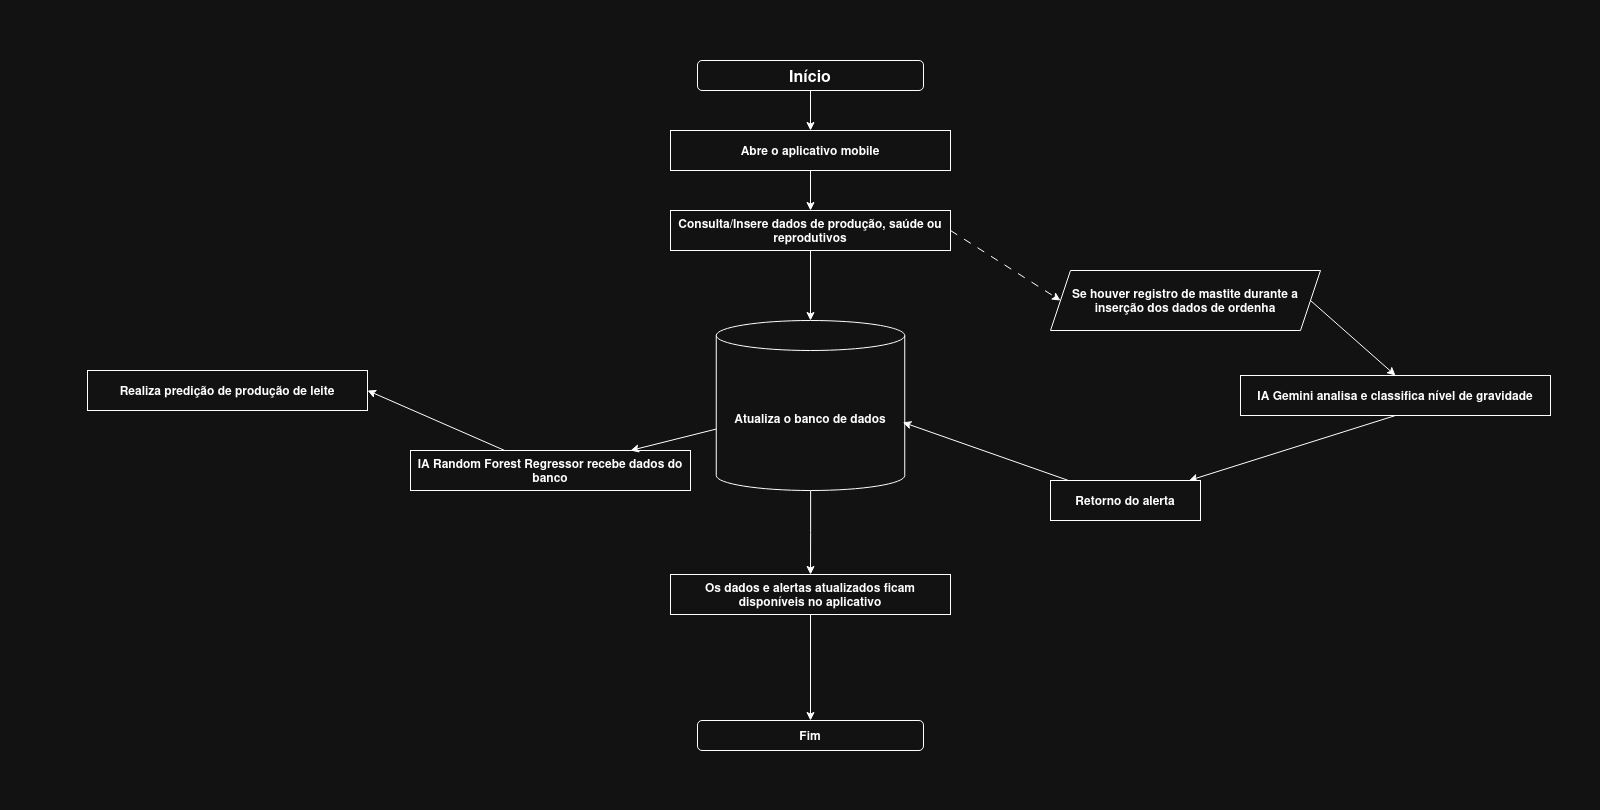
\includegraphics[scale=0.25]{diagrama_funcionario}
\SourceOrNote{Autoria Própria (2025)}
\end{flowchart}

Já no \Cref{fcht:fluxograma2}, o usuário acessa a plataforma web, onde são disponibilizados painéis interativos que apresentam indicadores consolidados de produtividade, sanidade e distribuição do rebanho. Nessa interface, o gestor pode consultar o prontuário individual dos animais, visualizar as predições geradas pela IA de regressão e acompanhar os alertas oriundos da análise de mastite. Caso necessário, é possível inserir ou atualizar informações diretamente pela plataforma web, mantendo a consistência do banco de dados sem a necessidade de acesso ao aplicativo móvel. Essa estrutura integrada permite que o gestor acompanhe em tempo real o desempenho produtivo da propriedade, utilizando dados concretos e análises automatizadas para fundamentar suas decisões de manejo e de investimento.
\newpage
\begin{flowchart}[!htb]
\centering
\caption{Fluxograma visão do Proprietário/Gestor}%
\label{fcht:fluxograma2}
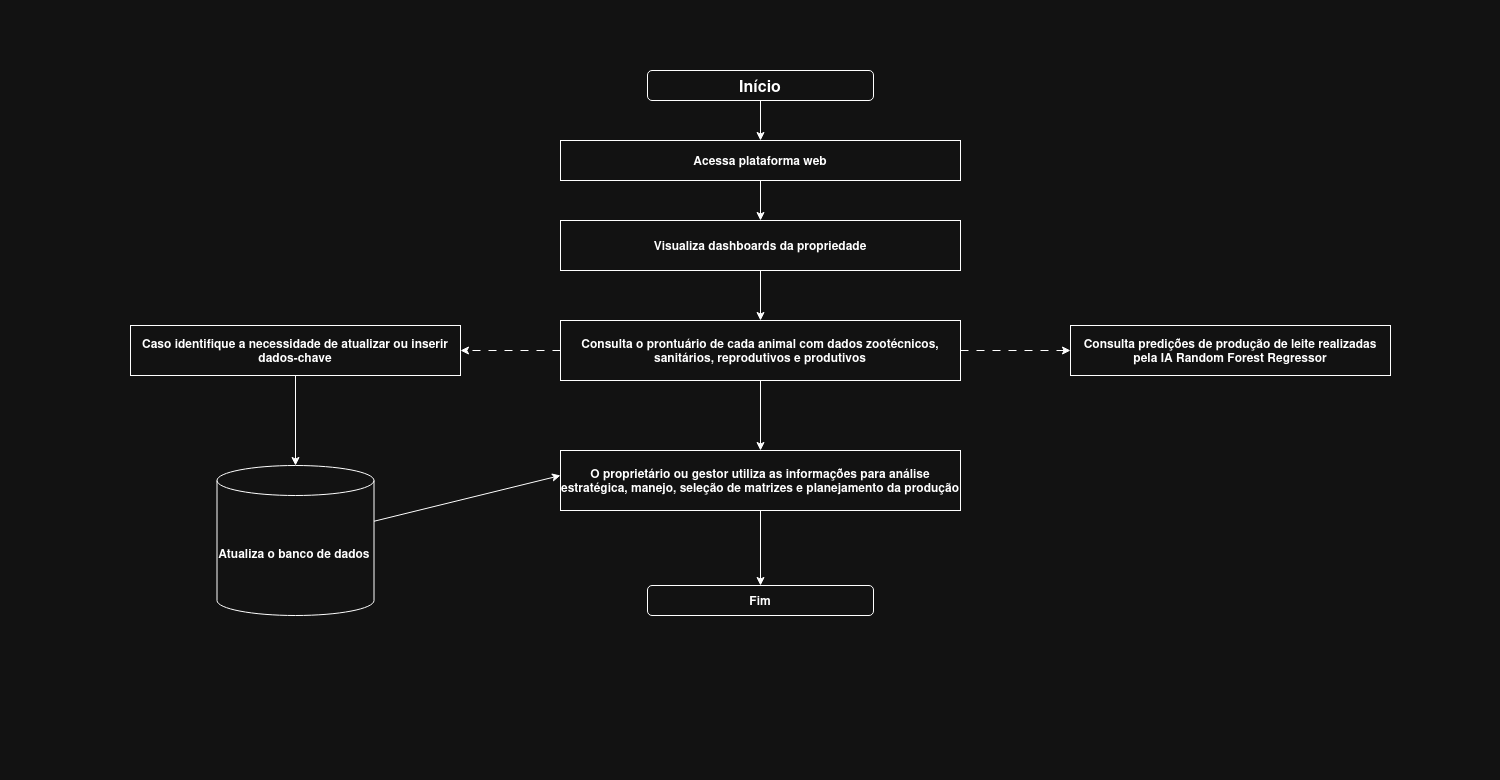
\includegraphics[scale=0.25]{diagrama_propreitario}
\SourceOrNote{Autoria Própria (2025)}
\end{flowchart}

Foi apresentado, anteriormente, toda a fundamentação teórica referente ao fluxo de funcionamento do sistema. Para que esse fluxo ocorra de forma adequada, é necessário o uso de um conjunto de ferramentas e tecnologias que viabilizam a comunicação entre as diferentes camadas da aplicação, conforme ilustrado na \Cref{fcht:arquitetura}. A interação com o usuário inicia-se nas etapas I e II. A Etapa I corresponde à plataforma web, desenvolvida em \textit{React} com o framework \textit{Next.js}. Atualmente, essa plataforma encontra-se hospedada na Vercel, uma solução \textit{serverless} que dispensa a necessidade de um servidor dedicado. A Etapa II refere-se à plataforma mobile, desenvolvida em \textit{React Native}, framework que consiste em um conjunto de ferramentas voltadas à criação de aplicações móveis nativas \cite{Bruna2021}. O aplicativo tem como principal funcionalidade oferecer uma interface simplificada e intuitiva, voltada ao lançamento de dados em campo.

Ambas as plataformas comunicam-se com o Back-end (etapa III) por meio de uma API, desenvolvida em \textit{TypeScript} com o framework \textit{Nest.js}. Como parte do Back-end, foram implementados recursos adicionais com o objetivo de aperfeiçoar a usabilidade e a fluidez do sistema, destacando-se a integração com dois modelos de Inteligência Artificial(IA). A primeira delas é a API \textit{Gemini} (etapa V), um modelo generativo multimodal desenvolvido pelo Google. No contexto deste projeto, a \textit{Gemini} é utilizada no sistema de alertas, por meio do modelo \textit{gemini-1.5-flash}. Essa implementação analisa um \textit{prompt} elaborado especificamente para o domínio do sistema e define a prioridade de cada alerta como alta, média ou baixa, simplificando de maneira significativa a lógica de priorização e resposta.

A segunda IA (etapa IV) foi desenvolvida pelo próprio grupo e baseia-se no algoritmo \textit{Random Forest Regressor}, um método de aprendizado supervisionado que combina múltiplas árvores de decisão para realizar previsões numéricas. O modelo é treinado com diversas amostras aleatórias dos dados e, para cada árvore, um subconjunto de atributos, conhecidos como \textit{features}, é selecionado de forma aleatória, promovendo diversidade entre os estimadores. A predição final é obtida a partir da média dos resultados de todas as árvores, aumentando a precisão e reduzindo o risco de sobreajuste, conhecido como \textit{overfitting}, em comparação com o uso de uma única árvore de decisão. No contexto deste trabalho, o modelo tem como objetivo prever individualmente a produção de leite de cada fêmea, utilizando seu histórico produtivo, reprodutivo, sanitário, zootécnico e genético. Essas informações são consolidadas em um conjunto de \textit{features} estruturadas e, a partir delas, o sistema gera uma predição que classifica o potencial produtivo em categorias, sendo elas alto, bom, médio ou baixo. O resultado é ainda comparado com a média da propriedade e fornece informações adicionais, como o volume previsto em litros, o percentual em relação à média e a data da predição.

Para disponibilizar todo o Back-end de forma operacional e acessível, o mesmo foi hospedado na nuvem utilizando o serviço \textit{Amazon EC2}, \textit{Elastic Compute Cloud}, da \textit{Amazon Web Services} (AWS) (etapa VII). Essa escolha permite escalar a infraestrutura dinamicamente, otimizando custos e garantindo melhor desempenho do sistema. A API é responsável por gerenciar toda a lógica de negócios, incluindo a criação, consulta, atualização e exclusão de registros no banco de dados, além de processar requisições provenientes das plataformas web e mobile. O controle de \textit{deploy} automático (etapa VIII) é realizado por meio do \textit{GitHub Actions}, que integra diretamente com a instância EC2, automatizando atualizações e correções e assegurando que a aplicação permaneça sempre disponível e atualizada para os usuários.

Para o armazenamento das informações, o banco de dados do sistema (etapa VI) foi desenvolvido em \textit{PostgreSQL}, escolhido pela sua robustez e pela consistência oferecida pelo modelo relacional na organização e integridade dos dados. Essa estrutura permite armazenar grandes volumes de informações de forma estruturada, garantindo que registros relacionados, como dados de produção, lactação e histórico sanitário dos animais, sejam mantidos de forma segura e coerente. Atualmente, o banco de dados encontra-se hospedado na nuvem por meio da plataforma \textit{Supabase}, que oferece compatibilidade nativa com o PostgreSQL, além de recursos adicionais de autenticação e armazenamento.

\begin{flowchart}[!htb]
\centering
\caption{Arquitetura do fluxo das redes}%
\label{fcht:arquitetura}
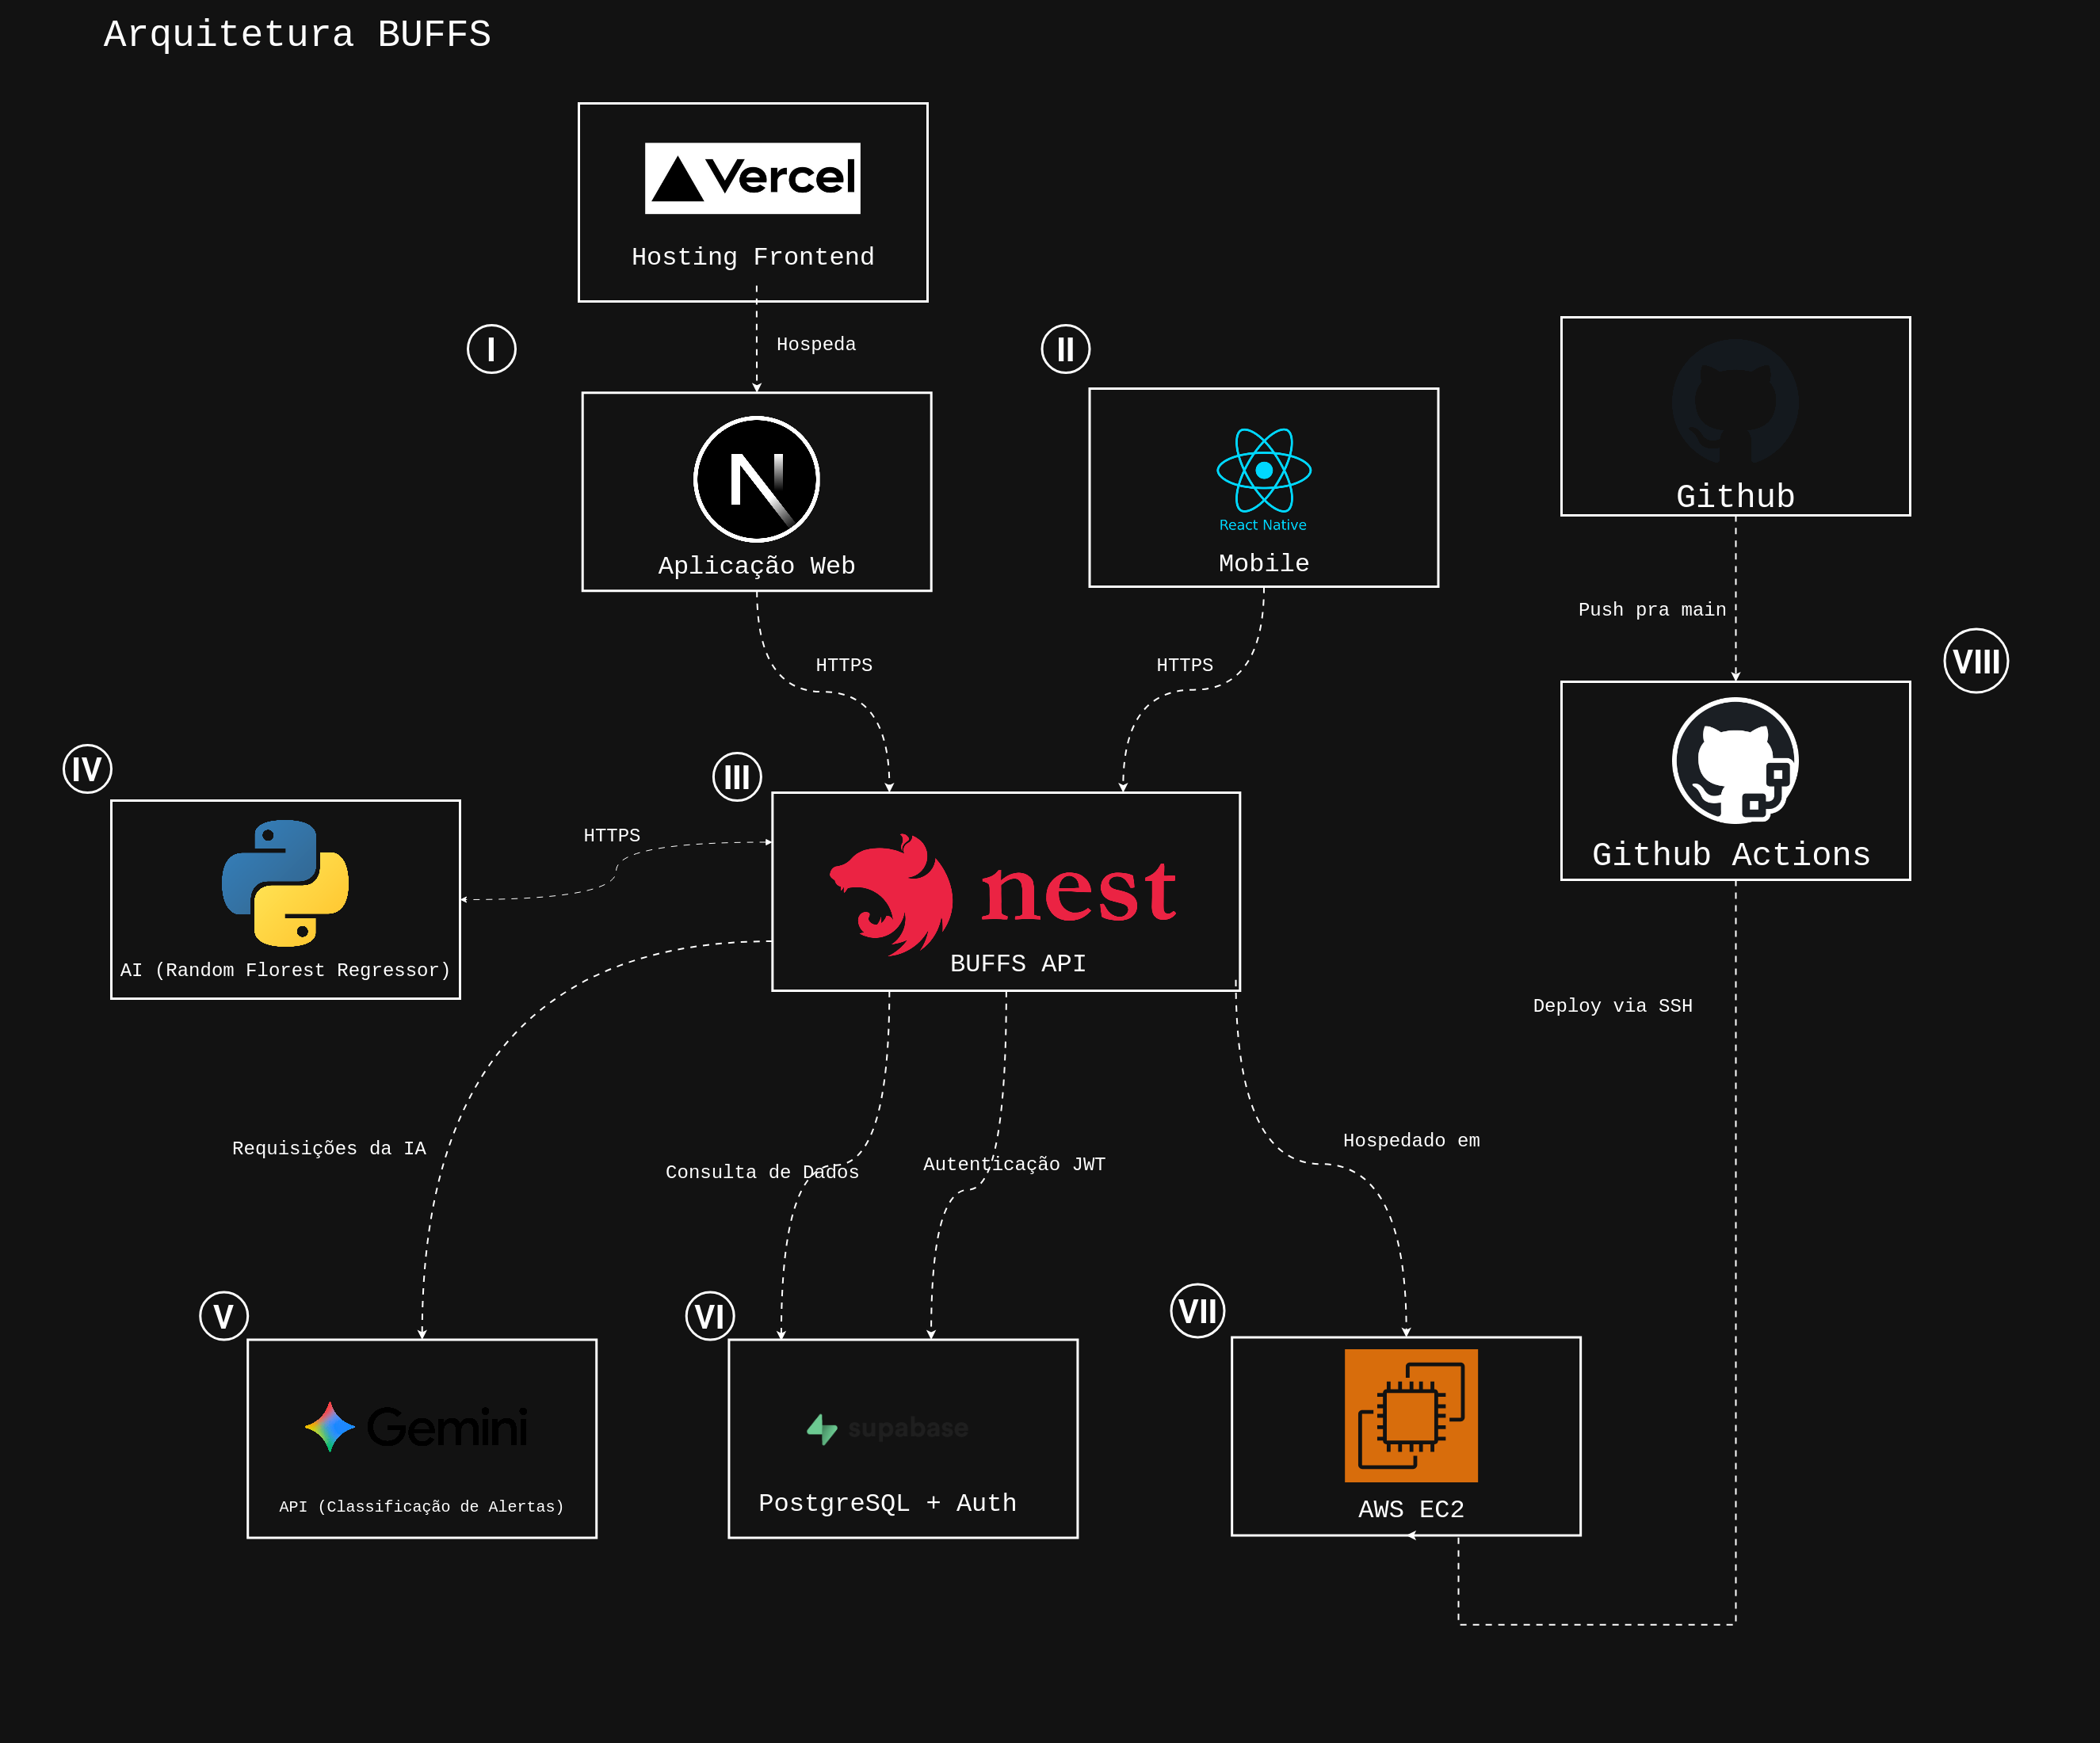
\includegraphics[scale=0.15]{buffs-arch-model}
\SourceOrNote{Autoria Própria (2025)}
\end{flowchart}

Após a análise do fluxo apresentado, nota-se que grande parte do sistema encontra-se hospedada na nuvem, seja por meio de serviços \textit{serverless}, bancos de dados em ambiente \textit{cloud} ou máquinas virtuais dedicadas. Essas escolhas, no momento atual, mostraram-se adequadas sob a ótica do grupo, uma vez que permitem distribuir as \textit{stacks} entre diferentes serviços, evitando a sobrecarga de um único sistema. Além disso, essa configuração possibilita a realização de testes de forma gratuita, sem a necessidade de investimentos iniciais em infraestrutura. Outro fator determinante nas decisões de arquitetura foi o alinhamento com os conteúdos abordados em sala de aula, privilegiando tecnologias e metodologias com as quais o grupo possui maior afinidade e embasamento técnico. Essa estratégia busca não apenas consolidar o aprendizado adquirido ao longo do curso, mas também garantir que o desenvolvimento ocorra de maneira segura e fundamentada em conhecimentos previamente assimilados.


%\section*{RESULTADOS PRELIMINARES}\label{sect:resultados}%

%Para avaliar a eficácia do modelo de IA desenvolvido para o sistema, foram realizadas análises comparativas entre as predições geradas e os valores reais de produção de leite. Com o desenvolvimento da IA baseada no modelo Random Forest Regressor, o desempenho do sistema foi avaliado por meio do coeficiente de determinação (\(R^2\)), obtendo-se o valor de 0,73. Como mostrado no Gráfico \Cref{grph:example}, a dispersão das predições em relação aos valores reais indica que a maior parte das estimativas se aproxima da diagonal \(y = x\), evidenciando que o modelo consegue explicar 73\% da variabilidade observada na produção de leite. Apesar de alguns desvios individuais, os resultados demonstram que o sistema fornece previsões consistentes e confiáveis para o manejo do rebanho.  O modelo considera informações como dias em lactação, produção média de lactação, histórico da produção média, idade da búfala, idade no primeiro parto e intervalo entre partos, permitindo análises detalhadas e suporte à tomada de decisão baseada em dados.

\begin{graph}[!h]
\centering
\SetCaptionWidth{\ifbool{@LayoutA}{0.47}{0.49}\linewidth}
\caption{Dispersão das predições do modelo}%
\label{grph:example}
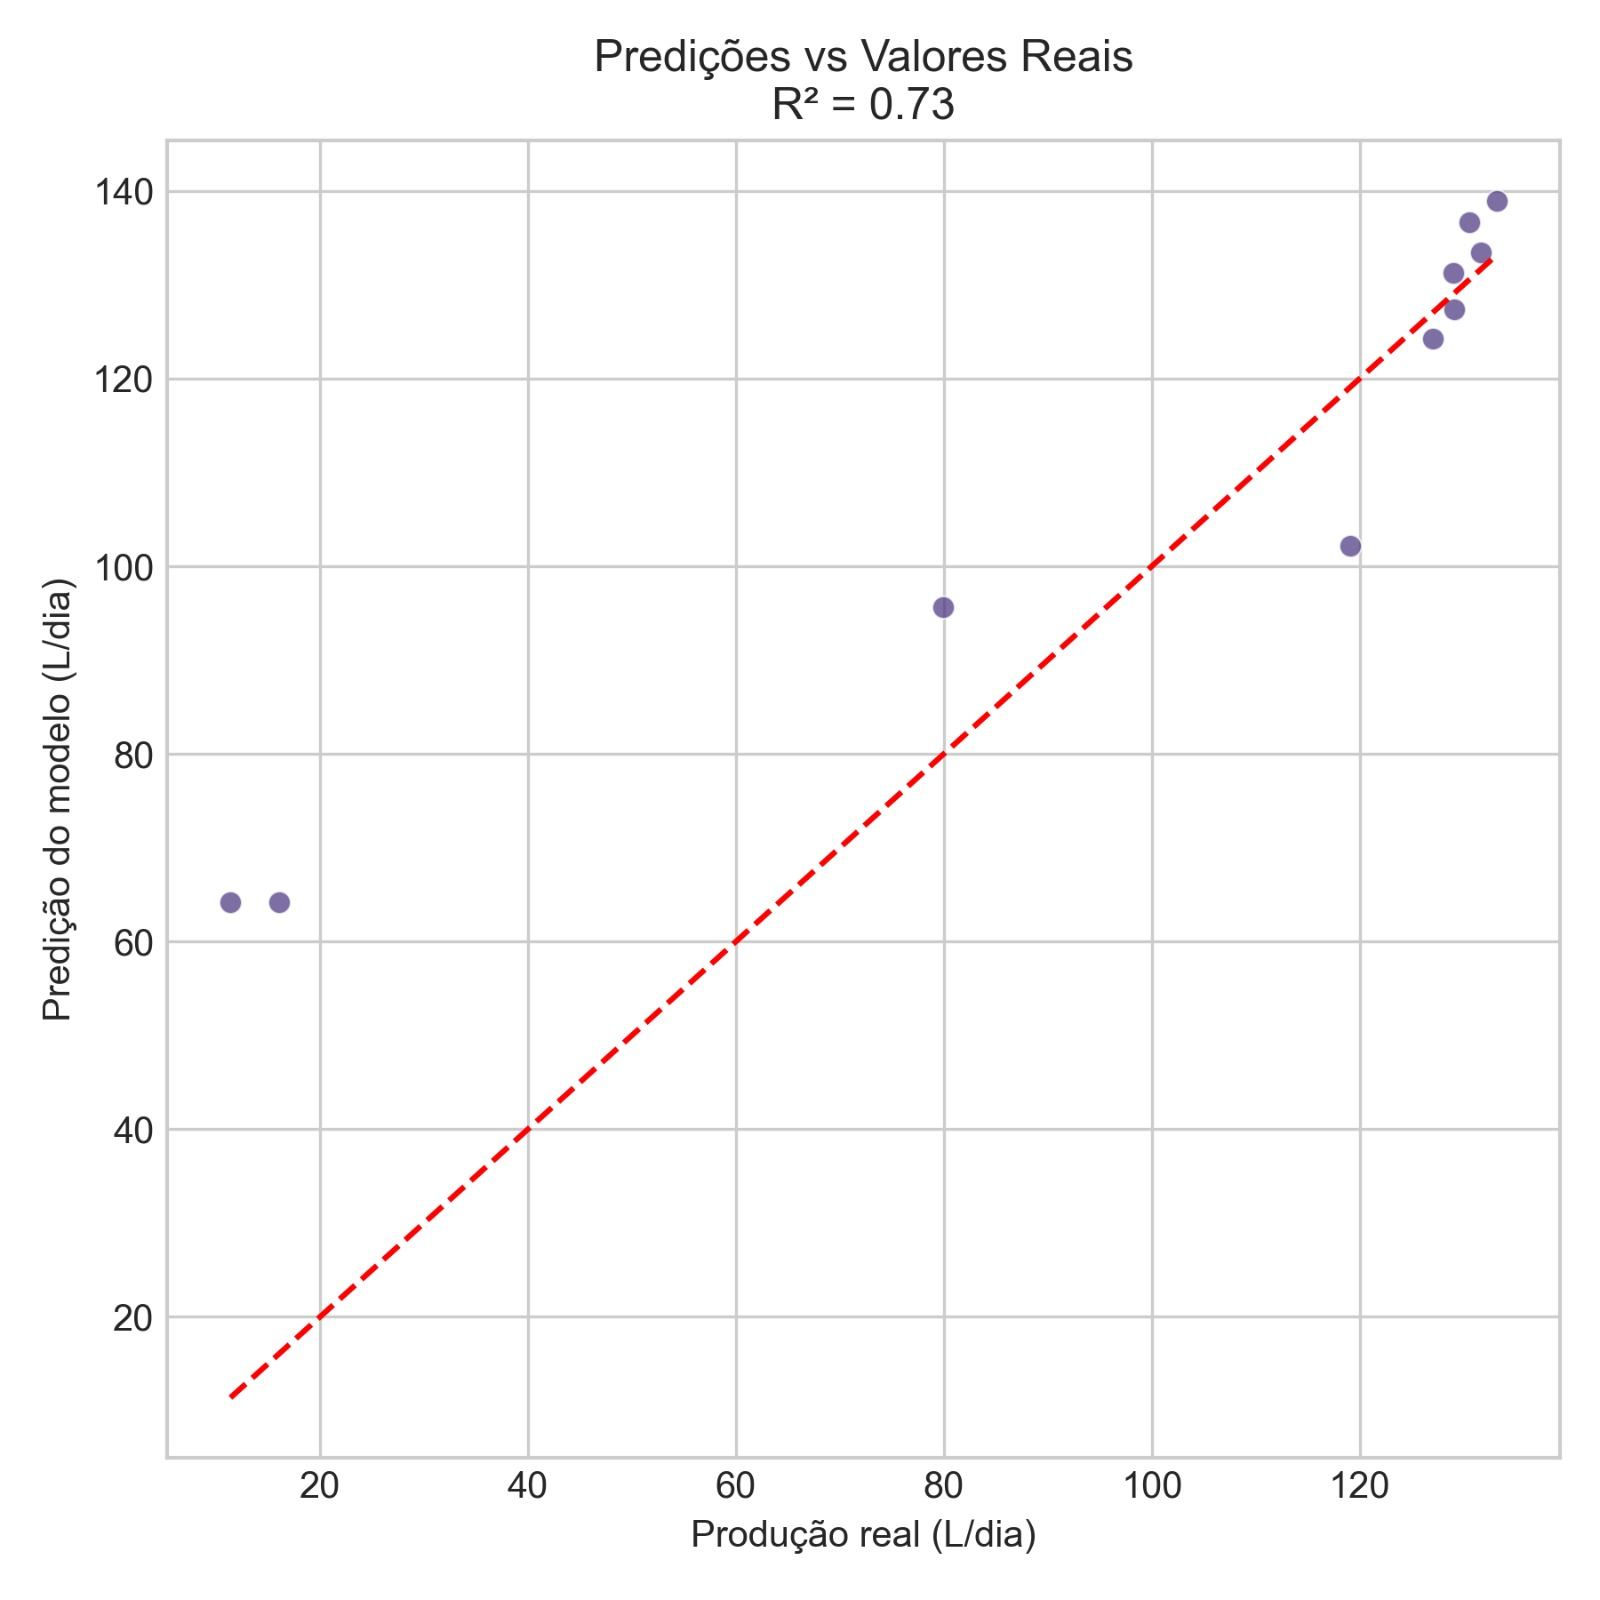
\includegraphics[width = \CaptionWidth]{R}
\SourceOrNote{Autoria Própria (2025)}
\end{graph}
%

%\section*{CONCLUSÃO}\label{sect:conclusao}%

%O desenvolvimento da plataforma demonstrou avanços significativos na organização e registro das informações zootécnicas, sanitárias, reprodutivas e produtivas do rebanho. Ao substituir planilhas e anotações manuais, a aplicação oferece uma interface simplificada e intuitiva, permitindo que os usuários registrem, consultem e analisem dados de maneira ágil e organizada. Essa melhoria reduz erros de registro, aumenta a consistência das informações e facilita o acesso a históricos completos de cada animal.

Embora a separação de funções entre as plataformas web e mobile apresente grande potencial, atualmente a versão mobile possui uma limitação quanto à disponibilidade, estando acessível apenas em dispositivos com sistema operacional Android.

O sistema já foi populado com dados reais fornecidos pelo Instituto de Zootecnia, permitindo validar sua funcionalidade e a integração com o banco de dados principal. No entanto, é necessário realizar testes prolongados em produção, uma vez que a geração contínua e a manutenção dos dados precisam ser avaliadas para estimar os custos de hospedagem e confirmar o desempenho em larga escala.

A inteligência artificial, implementada por meio do modelo Random Forest Regressor, foi utilizada para fornecer predições da produção de leite de cada animal, considerando informações históricas e características individuais. O modelo atingiu um coeficiente de determinação (R²) de 0,73, demonstrando que consegue explicar a maior parte da variabilidade observada na produção de leite. Esse desempenho evidencia que a IA é adequada para uso prático, fornecendo estimativas confiáveis que podem subsidiar decisões de manejo, sem substituir o julgamento do gestor ou veterinário.

Dessa forma, o projeto Buffs apresenta grande potencial para se tornar o primeiro sistema voltado especificamente para o manejo de bubalinos, contribuindo para que propriedades rurais aumentem a eficiência e a produtividade do rebanho.
%

\printbibliography

%% Elementos pós-textuais (opcionais): Apêndice e Anexo
%Caso for utilizar, basta retirar o símbolo de % na frente do comando
%%%%% Elementos pós-textuais
%%
%% Glossário, apêndices, anexos e índice remissivo (opcionais).

%% Apêndices
\begin{Appendix}

\section{Título de Apêndice}%
\label{sect:apx-a1}

Exemplo de apêndice (\Cref{sect:apx-a1}) em uma seção de \nameref{sect:appendix}.

\subsection{Título de Seção Secundária de Apêndice}%
\label{ssect:apx-a2}

Exemplo de seção secundária de apêndice (\Cref{ssect:apx-a2}).

\subsubsection{Título de Seção Terciária de Apêndice}%
\label{sssect:apx-a3}

Exemplo de seção terciária de apêndice (\Cref{sssect:apx-a3}).

\paragraph{Título de seção quaternária de Apêndice}%
\label{prgh:apx-a4}

Exemplo de seção quaternária de apêndice (\Cref{prgh:apx-a4}).

\subparagraph{Título de seção quinária de Apêndice}%
\label{sprgh:apx-a5}

Exemplo de seção quinária de apêndice (\Cref{sprgh:apx-a5}).

\end{Appendix}

%% Anexos
\begin{Annex}

\section{Título de Anexo}%
\label{sect:anx-a1}

Exemplo de anexo (\Cref{sect:anx-a1}) em uma seção de \nameref{sect:annex}.

\subsection{Título de Seção Secundária de Anexo}%
\label{ssect:anx-a2}

Exemplo de seção secundária de anexo (\Cref{ssect:anx-a2}).

\subsubsection{Título de Seção Terciária de Anexo}%
\label{sssect:anx-a3}

Exemplo de seção terciária de anexo (\Cref{sssect:anx-a3}).

\paragraph{Título de seção quaternária de Anexo}%
\label{prgh:anx-a4}

Exemplo de seção quaternária de anexo (\Cref{prgh:anx-a4}).

\subparagraph{Título de seção quinária de Anexo}%
\label{sprgh:anx-a5}

Exemplo de seção quinária de anexo (\Cref{sprgh:anx-a5}).

\end{Annex}

%% Índice remissivo
\printindex%


%% Fim do documento
\end{document}